\chapter{Sensor tests}

%\section{Digital}
%    \subsection{Interface tests}
%    \subsection{Software tests}

\section{Power}
    \subsection{LDO stabilisation}
        Voltage after LDO was measured in time, to calculate delay between power enable and measurement start. Time graph is shown on figure \ref{LDO_rise_time}. Delay was estimated to be around \SI{1}{\second}.

        \begin{figure}[H]
            \centering
            \includegraphics[width=0.8\paperwidth]{img/07/rise_time.png}
            \caption{LDO rise time}
            \label{LDO_rise_time}
        \end{figure}

    \subsection{Power consumption}

\section{Current source}
    Current source was tested on HP 34970A - 6 1/2 digit multimeter, with 200 PLC enabled.

    \subsection{Noise}
        Noise of current source was measured for long period of time, taking sufficient number of samples. Results (\ref{Current_Stability}) shows that noise floor is below specifications for this meter.

        \begin{table}[H]
            \begin{center}
                \begin{tabular}{cc}
                    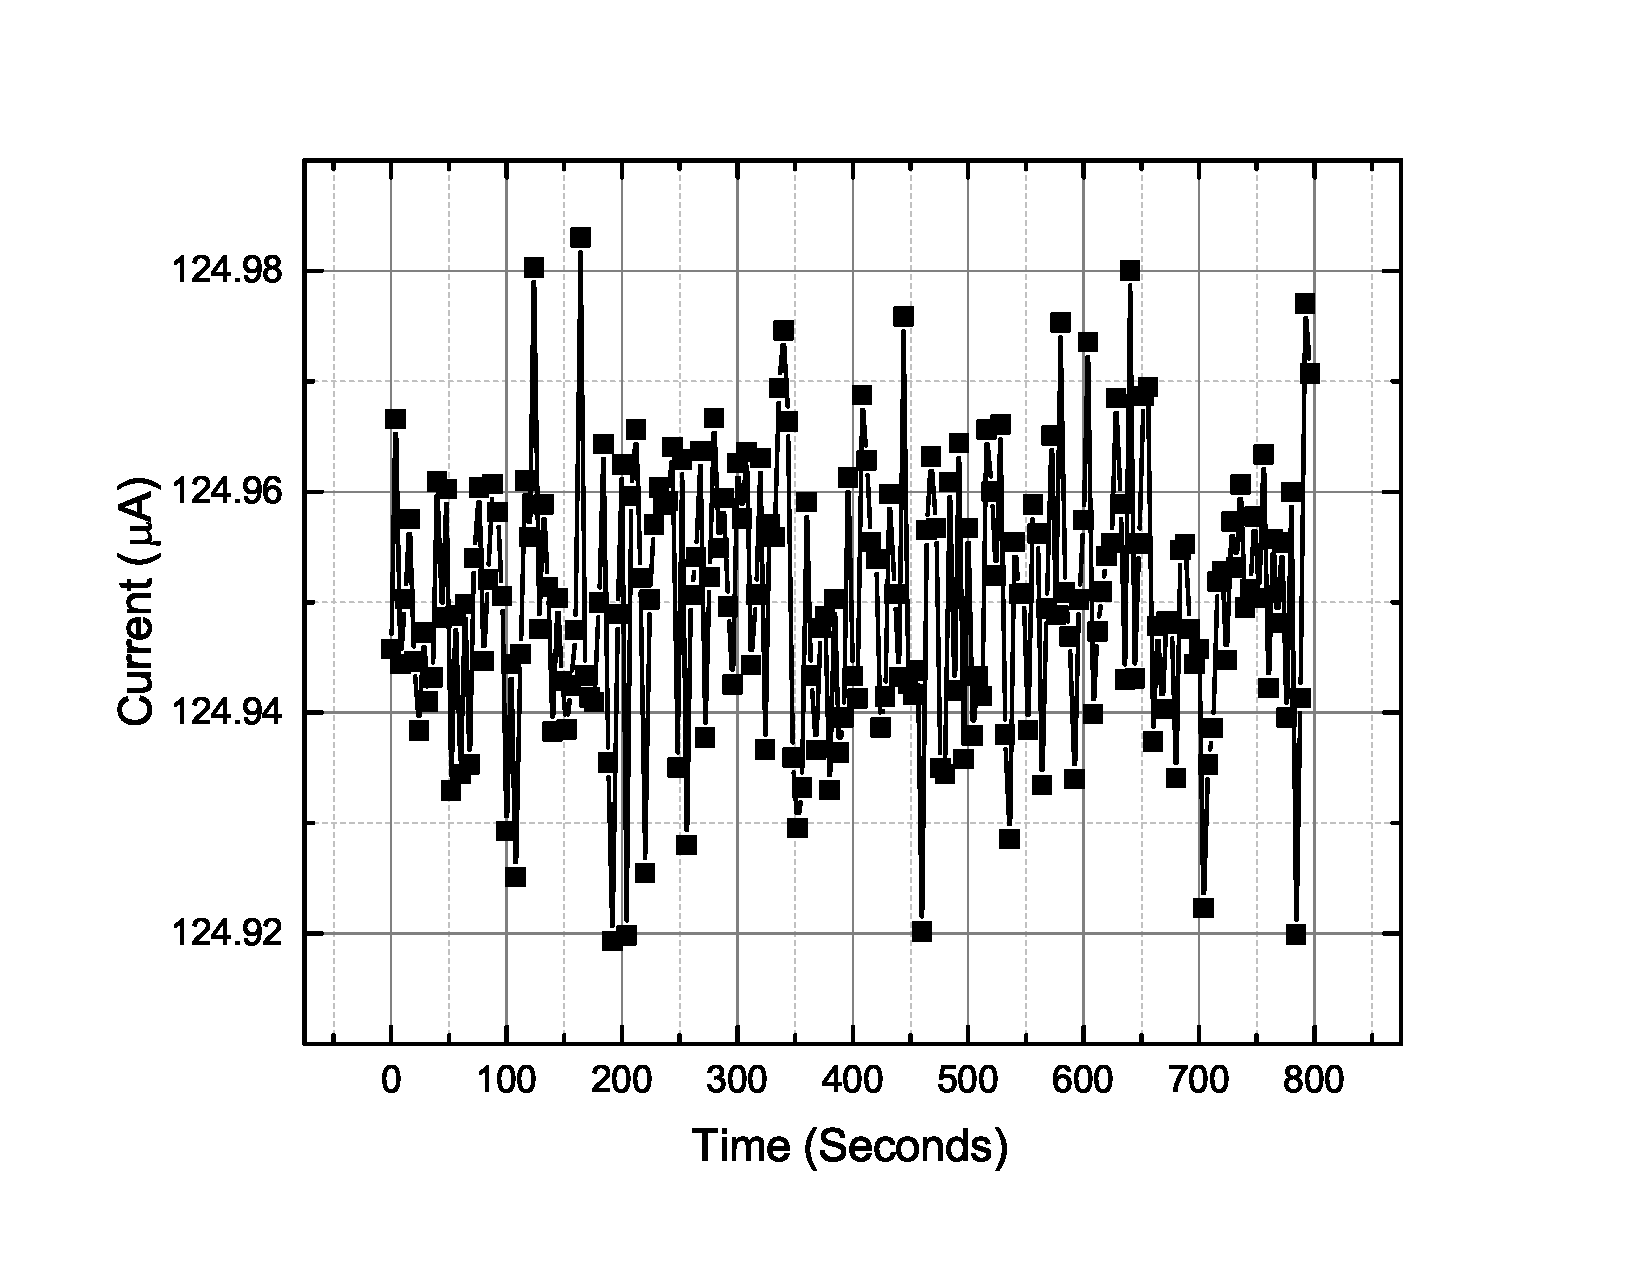
\includegraphics[width=0.35\paperwidth]{img/07/current_time.eps}
                    &
                    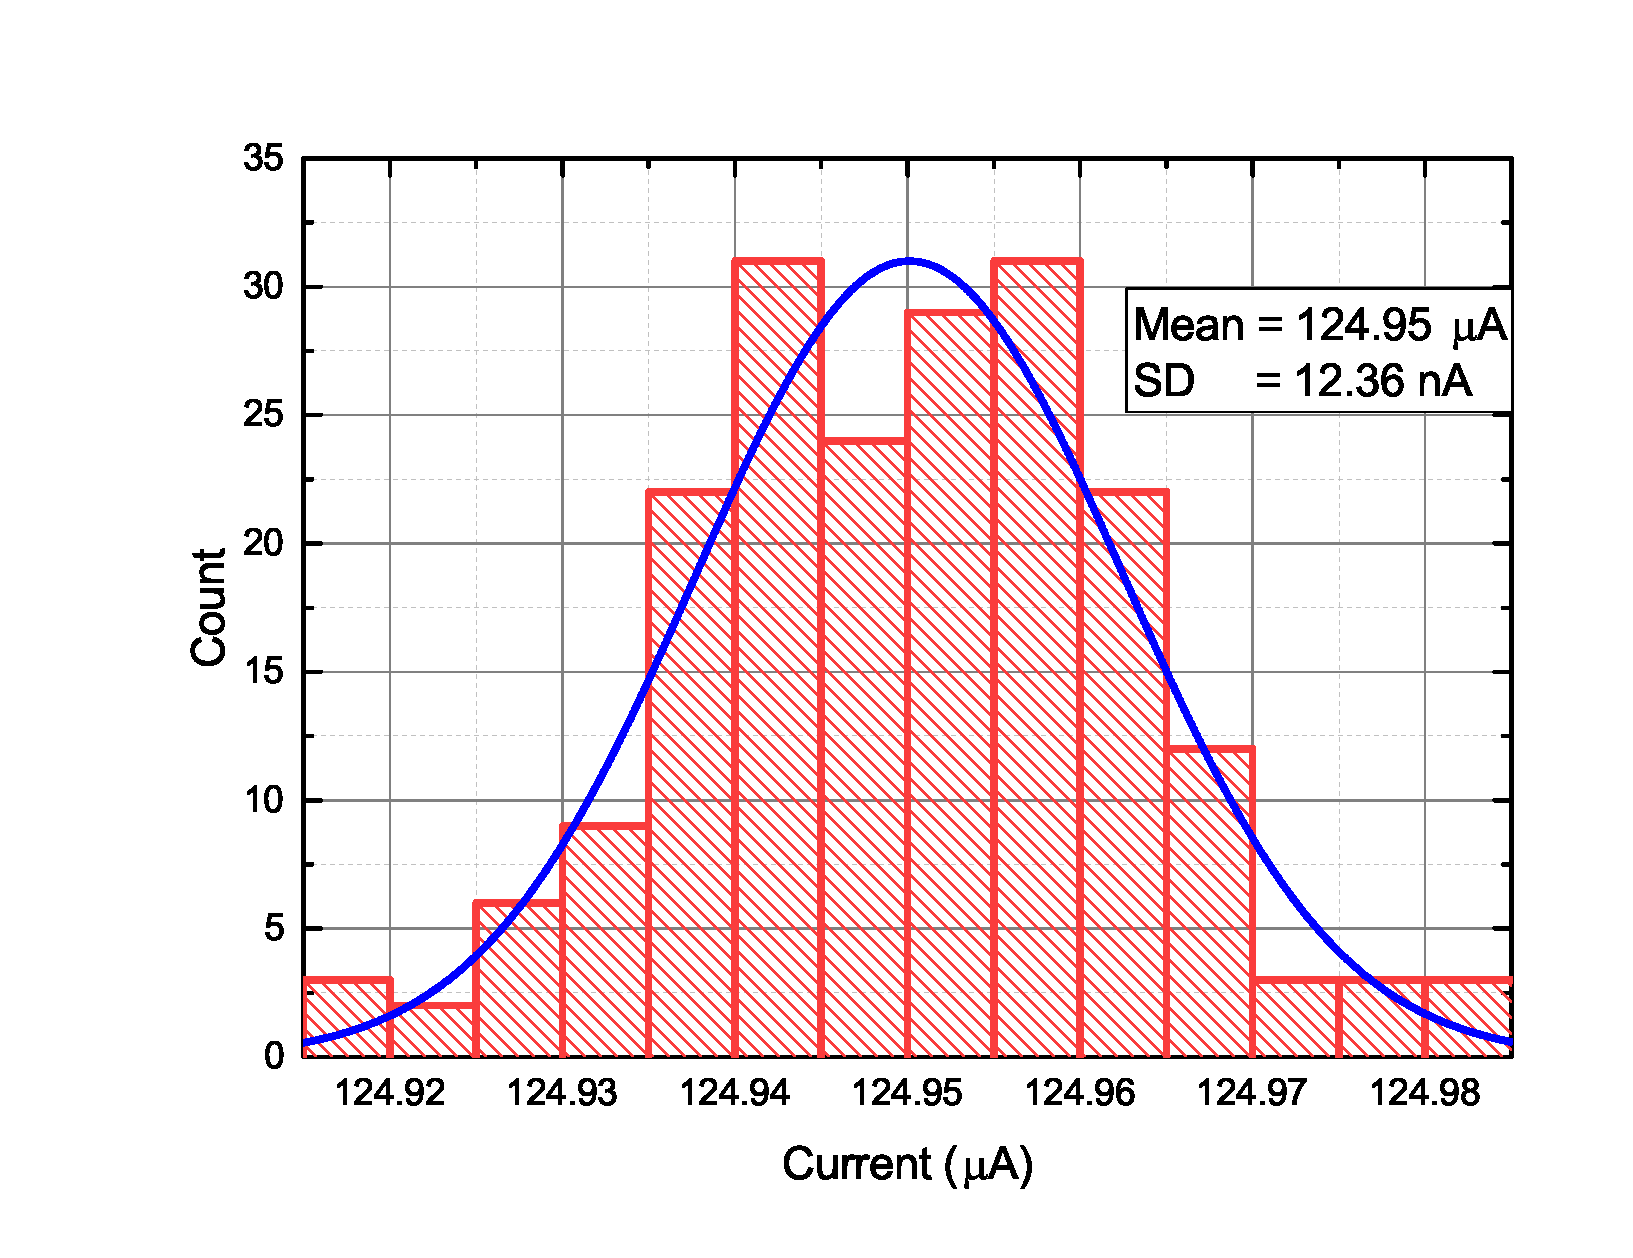
\includegraphics[width=0.35\paperwidth]{img/07/current_hist.eps}
                \end{tabular}
            \end{center}
            \caption{Current noise in time and histogram}
            \label{Current_Stability}
        \end{table}

    \subsection{Load range}
        Output load was changed in identical manner as in simulation, to tests its fidelity. Simulation and build model shown same range and stability - confirming the design. Current source works as intended for loads between \SI{1.4}{\kilo\ohm} and \SI{22.5}{\kilo\ohm} (figure \ref{Current_sensor_output_characteristics}).
        \begin{figure}[H]
            \centering
            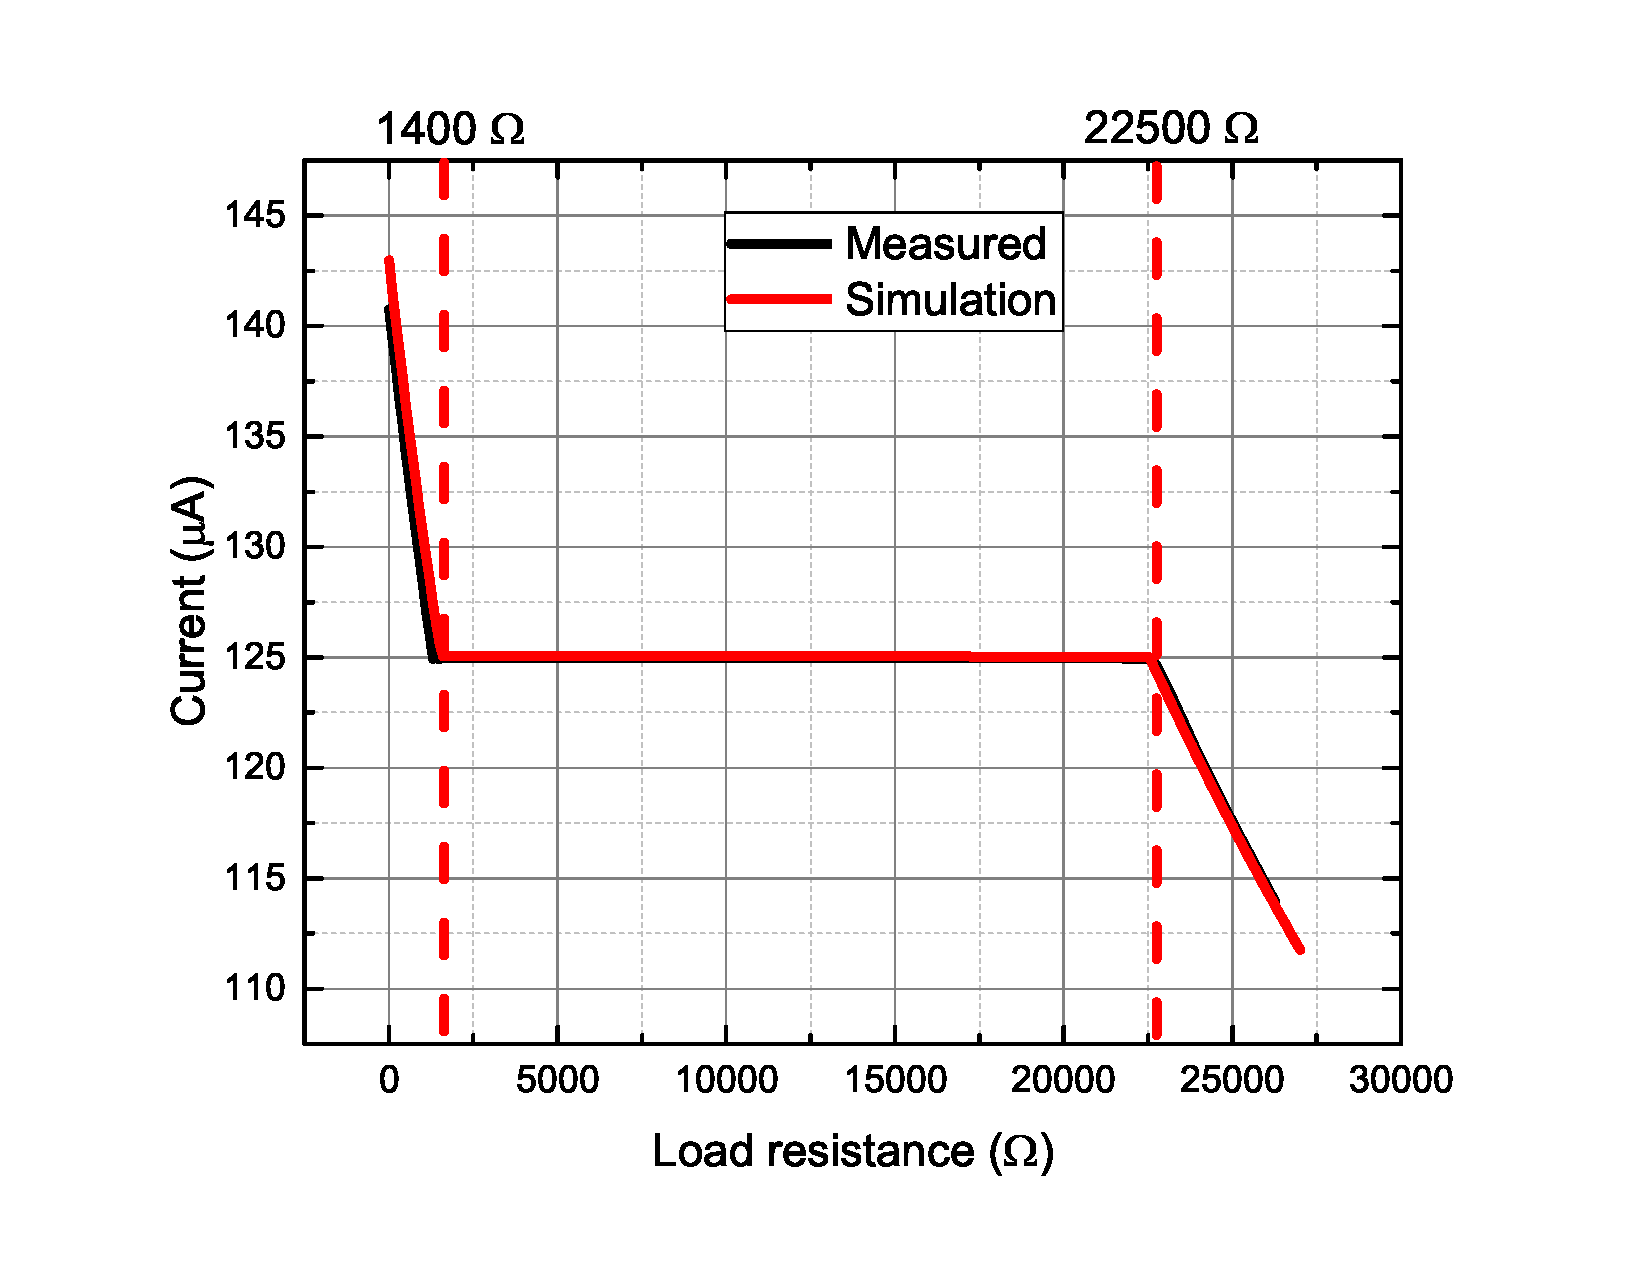
\includegraphics[width=0.6\paperwidth]{img/07/output_resistance.eps}
            \caption{Current sensor output characteristics}
            \label{Current_sensor_output_characteristics}
        \end{figure}

    \subsection{Temperature stability}
        Temperature was swept from $20$ to \SI{70}{\degreeCelsius}, no detectable changes were measured by available meter, therefore it is assumed that current source changes lower than about \SI{20}{\nano\ampere} in this temperature range.

\section{MOS settling}
    After enabling measurement channel for threshold voltage it takes a lot of time to fully stabilize its value. Instead of pre-enabling, same time method was used. ADC takes measurement of threshold voltage at precisely specified time after enabling power. On figure \ref{MOS_settling} 10 runs of measured voltage vs time are plotted, proving this method is stable within \SI{20}{\uV}.

    \begin{figure}[H]
        \centering
        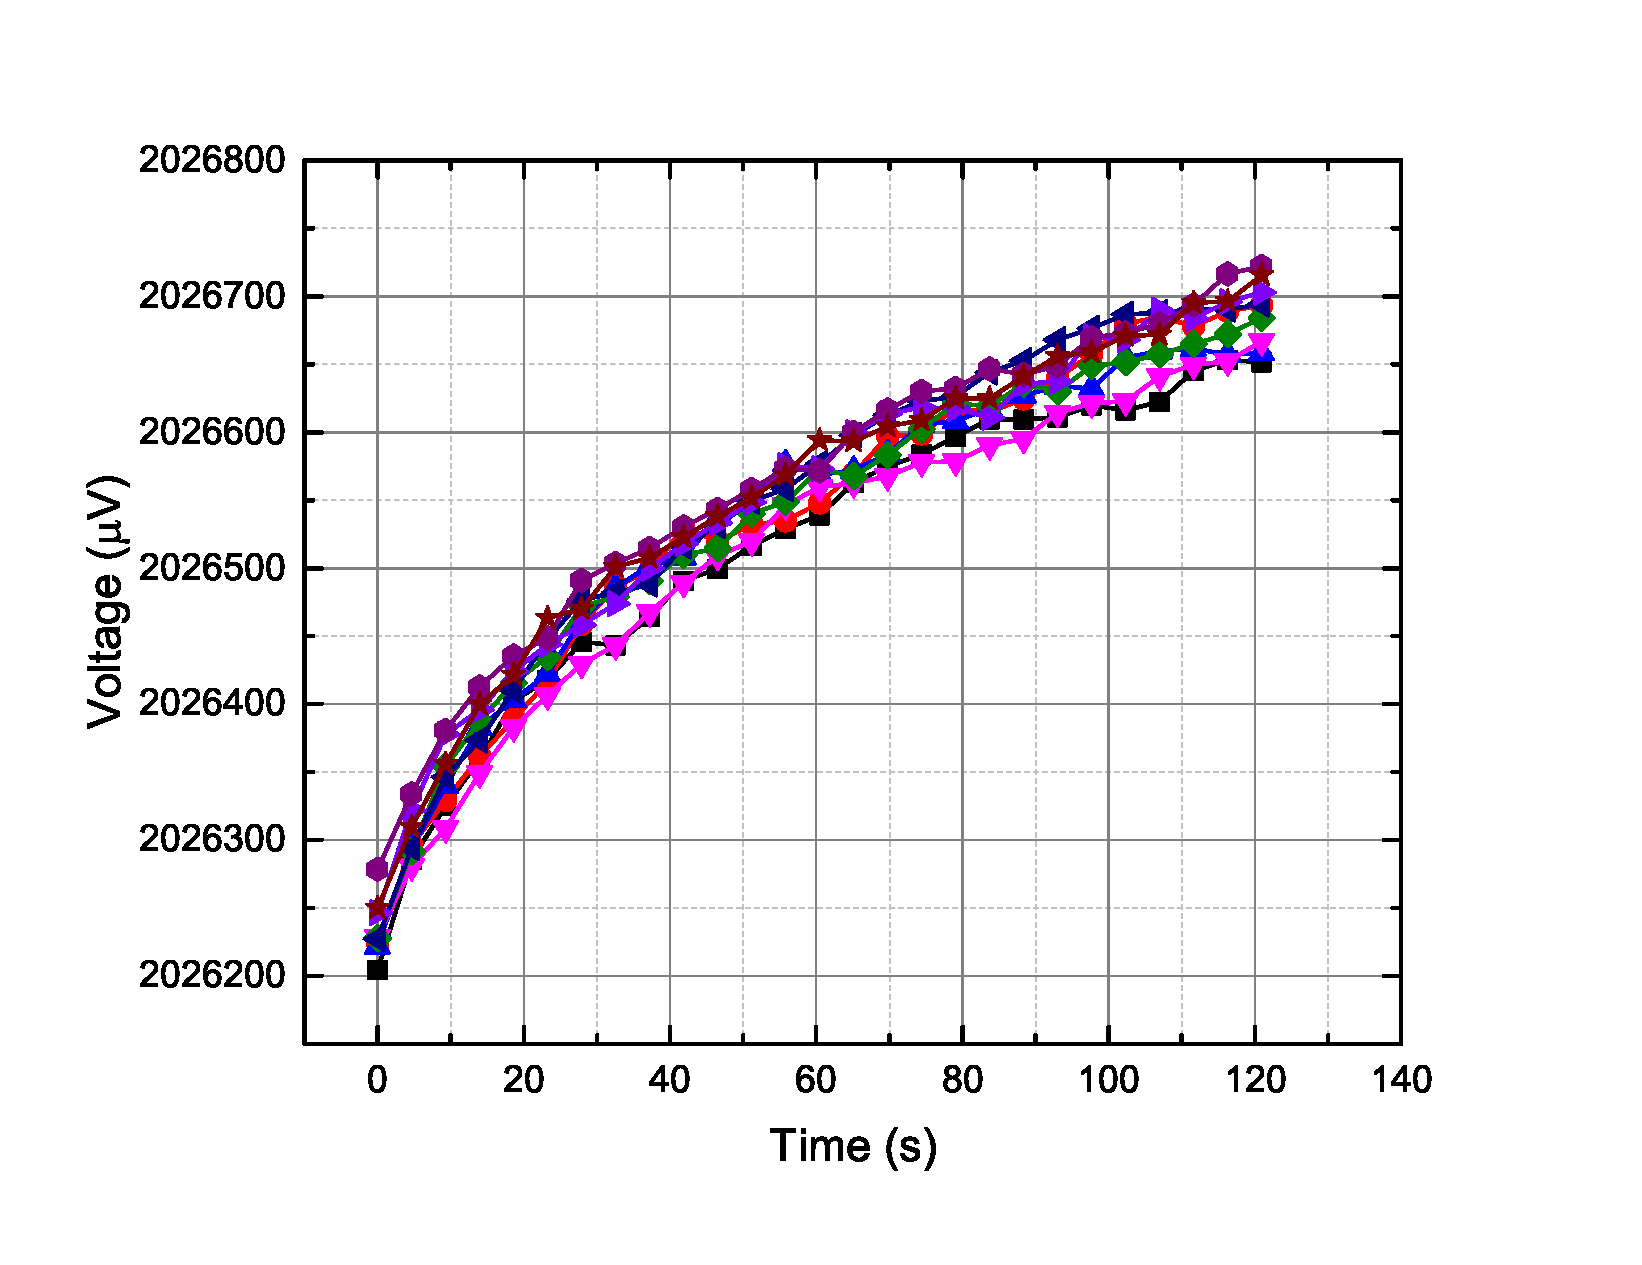
\includegraphics[width=0.8\paperwidth]{img/07/MOS_settling.eps}
        \caption{10 runs of MOS voltage setting}
        \label{MOS_settling}
    \end{figure}

\section{Measurement noise}
    Most important noise figure is system noise - ADC reading noise floor during nominal work.

    Because even smallest temperature changes cause ADC reading to shift (due to threshold/diode voltage shift) this efect had to be eliminated to measure noise. For this purpose DC notch filter was used in post-processing, to eliminate any DC bias during measurement. Transfer function of this filter is shown on figure TODO. Example of filtration is shown on figure TODO.

    Image: [przed filtracją] -> po filtracji

    Image: ch-ka filtru

    \subsection{Diode}
        Image: time + histogram

        Noise on temperature measurement channel have standard deviation of $1.2 uV$
    \subsection{Threshold voltage}
        Image: time + histogram

        Noise on threshold voltage measurement channel have standard deviation of $8.2 uV$

    \subsection{Interpretation}
        Because the only difference between temperature and threshold voltage channels is semiconductor itself, source of noise can be estimated from significant difference between them.

        Estimated current source noise is $2 nA$.
        This value can be confirmed by calculations, reference voltage LT1634 have low-frequency noise of $U_N = \SI{15}{\uV}$, this value is directly across series resistor, therefore $I_{NOISE} = U_N/R = \SI{1.5}{\nA}$. Noise output from LTSpice:



\section{Temperature characteristics}
    By sweeping temperature from \SI{0}{\degreeCelsius} up to \SI{75}{\degreeCelsius} temperature dependency charts were obtained for the device.

    \subsection{Diode}
        Diode response (ref) is alsost ideally linear.

        Image: chart + dopasowanie

    \subsection{Threshold voltage}
        Threshold voltage (ref) tends to be non-linear, but quadratic equation can be fitted to it.

        Image: chart + dopasowanie


\section{Temperature compensation stability}
    The sensor should be compensated for temperature, with assumption that temperature characteristic curves will not change during irradiation.

    During temperature sweep data was gathered, and post-processed applying thermal compensation (given by charts ref and ref). In full sensing range, sensor output shifts of maximum $\SI{400}{\uV}$, which reflects to TID measurement accuracy of \SI{\pm 1}{\rad}.



    
